\secnumbersection{PROPUESTA DE SOLUCIÓN}

% Se debe desarrollar la solución propuesta. Los subcapítulos por poner aquí son propios del autor. Se sugiere mencionar metodología usada. Es conveniente incorporar figuras y tablas para aclarar la solución, que deben indicar el número de la figura, su nombre y su autor o fuente (si las diseñas tú, la fuente es ``Elaboración propia''). Ver ejemplos en esta página y en la siguiente.

% Cabe mencionar que aquí está la esencia del trabajo en lo que se refiere al aporte creativo del memorista, es el momento de demostrar que usted es un destacado profesional que creó, diseñó y/o llevó a cabo la solución propuesta.

Esta propuesta presenta la evolución de \textbf{DRAFTS} \cite{zhang2024drafts} desde un prototipo de investigación hacia un \textit{pipeline} \textbf{productivo, robusto y eficiente} diseñado para operaciones observacionales a gran escala. La transformación arquitectónica no se limita a mejoras incrementales, sino que establece una \textbf{extensión fundamental para regímenes de alta frecuencia} que expande significativamente las capacidades de detección en el espectro milimétrico.

\subsection{Vista General: Dos Grandes Bloques de Contribución}

Esta propuesta se estructura en \textbf{dos grandes bloques} que abordan desafíos complementarios en la detección de FRBs:

\textbf{Bloque 1: DRAFTS++ - Pipeline Productivo, Robusto y Eficiente} aborda la transformación del prototipo DRAFTS original hacia un sistema productivo capaz de operar en entornos observacionales reales. Este bloque incluye la refactorización arquitectónica completa, implementación de procesamiento eficiente por chunks, trazabilidad completa y artefactos de salida estandarizados.

\textbf{Bloque 2: Extensión a Alta Frecuencia - Cuatro Líneas de Investigación} explora estrategias metodológicas para extender las capacidades de detección hacia regímenes de alta frecuencia (30-100 GHz), donde las firmas dispersivas tradicionales se atenúan significativamente. Este bloque presenta cuatro líneas de investigación complementarias que abordan diferentes aspectos del desafío de detección en el espectro milimétrico.

\subsection{Bloque 1: DRAFTS++ - Pipeline Productivo, Robusto y Eficiente}

Este bloque aborda la transformación fundamental del prototipo DRAFTS original hacia un sistema productivo capaz de operar en entornos observacionales reales. La evolución desde un prototipo de investigación hacia sistema productivo requiere una transformación arquitectónica fundamental que aborde las limitaciones inherentes del código base original.

\subsubsection{Desafíos del Prototipo Original}

El prototipo inicial presenta una estructura monolítica con scripts independientes (\texttt{d-center-main.py}, \texttt{d-resnet-main.py}) optimizados para condiciones de laboratorio controladas pero incapaces de manejar la variabilidad operacional de entornos observacionales reales. Las limitaciones principales incluyen:

\begin{itemize}
\item \textbf{Estructura monolítica:} Scripts independientes sin integración coherente
\item \textbf{Procesamiento limitado:} Lectura monolítica de archivos grandes sin gestión de memoria
\item \textbf{Falta de trazabilidad:} Ausencia de logging estructurado y reproducibilidad
\item \textbf{Salidas inconsistentes:} Figuras y reportes ad hoc sin estandarización
\item \textbf{Escalabilidad limitada:} Sin soporte para procesamiento distribuido o streaming
\end{itemize}

\subsubsection{Pipeline End-to-End Modular y Escalable}

\noindent\textbf{Transformación arquitectónica fundamental.} La evolución desde scripts monolíticos hacia un sistema modular escalable constituye una contribución arquitectónica fundamental que establece las bases para operaciones productivas a gran escala. Esta transformación implementa una arquitectura modular con componentes especializados que establecen separación clara de responsabilidades y interfaces estandarizadas.

La reestructuración arquitectónica elimina las limitaciones inherentes del prototipo original, caracterizado por scripts independientes sin integración coherente, y establece un flujo de datos unidireccional que garantiza consistencia operacional y facilita mantenimiento y extensibilidad del sistema.

Los módulos especializados incluyen:
\begin{itemize}
\item \textbf{Ingesta de datos:} Manejo unificado de formatos observacionales estándar
\item \textbf{Preprocesamiento:} Normalización, mitigación de interferencia y preparación de datos
\item \textbf{Propuesta de candidatos:} Estrategias intercambiables de detección
\item \textbf{Clasificación:} Redes neuronales para validación binaria
\item \textbf{Validación:} Verificación DM-aware y consistencia temporal
\item \textbf{Visualización:} Generación automática de productos diagnósticos
\end{itemize}

Esta arquitectura modular establece una interfaz unificada con sistemas de configuración validados que permiten control granular de todos los parámetros del pipeline, garantizando trazabilidad completa mediante semillas fijas, versiones y firmas criptográficas de datos y modelos.

\subsubsection{Manejo Robusto de Archivos FITS, Filterbank y PSRFITS}

\noindent\textbf{Integración multi-formato para interoperabilidad observacional.} La capacidad de procesar múltiples formatos de datos observacionales constituye un requisito fundamental para la operación en entornos observacionales reales, donde diferentes instrumentos y observatorios emplean estándares de almacenamiento diversos.

El sistema implementa detección automática de tipos de archivo y manejo unificado de formatos estándar en radioastronomía, incluyendo FITS (Flexible Image Transport System), PSRFITS (específico para pulsares) y Filterbank (formato de datos filtrados). Esta interoperabilidad elimina la necesidad de conversiones manuales previas y permite el procesamiento directo de datos de múltiples observatorios sin configuración específica.

La implementación de parsers especializados para cada formato garantiza la extracción correcta de metadatos observacionales críticos, incluyendo parámetros temporales, espectrales y de polarización, estableciendo una base sólida para el procesamiento posterior.

\subsubsection{Sistema de Análisis de Headers FITS y Filterbank Avanzado}

\noindent\textbf{Extracción automática de parámetros observacionales.} La determinación automática de parámetros observacionales desde metadatos constituye una mejora fundamental que elimina errores humanos en la configuración del pipeline y acelera significativamente el proceso de setup.

El sistema implementa algoritmos de extracción automática que analizan headers FITS y metadatos de archivos Filterbank para determinar parámetros críticos como resolución temporal, resolución espectral, longitud del archivo, configuración de frecuencias, y parámetros de polarización. Esta automatización garantiza la configuración correcta del pipeline sin intervención manual.

La validación automática de parámetros extraídos asegura la coherencia interna de los datos y detecta inconsistencias que podrían comprometer la calidad del análisis, estableciendo un sistema robusto de control de calidad en la fase inicial del procesamiento.

\subsubsection{Sistema de Streaming y Gestión de Memoria Inteligente}

\noindent\textbf{Procesamiento eficiente de observaciones de larga duración.} La limitación fundamental del prototipo original radica en su incapacidad para procesar observaciones de larga duración debido a restricciones de memoria. Esta mejora implementa una arquitectura de streaming con gestión inteligente de memoria que permite procesar observaciones de cualquier duración.

El sistema calcula dinámicamente el tamaño óptimo de chunks basado en la memoria disponible del sistema, implementando un presupuesto inteligente que reserva recursos para operaciones GPU y overhead del sistema. Esta aproximación garantiza que el procesamiento se mantenga dentro de los límites de memoria disponibles mientras maximiza la eficiencia computacional.

La implementación de streaming por chunks con solapamiento controlado permite procesamiento eficiente mediante gestión automática de memoria, eliminando las limitaciones del prototipo original y estableciendo las bases para el procesamiento de observaciones de larga duración típicas en radioastronomía.

\subsubsection{Sistema de Precisión y Continuidad Temporal Quirúrgica}

\noindent\textbf{Trazabilidad temporal absoluta para localización precisa de eventos.} Una contribución técnica fundamental es la implementación de un sistema de continuidad temporal quirúrgicamente precisa que garantiza trazabilidad absoluta de cada evento detectado. Este sistema opera en múltiples niveles:

\textbf{Contigüidad Perfecta de Slices:} El algoritmo de planificación de slices garantiza contigüidad perfecta mediante validaciones estrictas que aseguran que cada slice termina exactamente donde comienza el siguiente, eliminando solapamientos y huecos temporales. Se implementa un sistema de redondeo estable que evita inconsistencias de redondeo bancario.

\textbf{Trazabilidad Temporal Absoluta:} Cada chunk mantiene marcas de tiempo absolutas basadas en Modified Julian Date (MJD) extraídas directamente de los headers FITS, con correcciones aplicadas para desplazamientos de subintegraciones. El cálculo del tiempo exacto de cada slice se realiza mediante la fórmula:

\[
t_{\text{slice}} = t_{\text{chunk\_start}} + (\text{start\_idx} \times \text{dt\_ds})
\]

donde $\text{dt\_ds}$ es la resolución temporal decimada, garantizando que cada burst detectado tenga una marca temporal quirúrgicamente precisa.

\textbf{Manejo de Discontinuidades:} El sistema detecta automáticamente gaps en los datos mediante comparación entre índices esperados e índices reales, insertando padding temporal cuando es necesario para mantener continuidad perfecta.

\textbf{Validación de Continuidad:} Se implementa un sistema de pruebas automatizadas que verifica contigüidad de índices, incrementos temporales exactos y coherencia entre chunks, usando tolerancias temporales basadas en la resolución instrumental.

\begin{figure}[H]
\centering
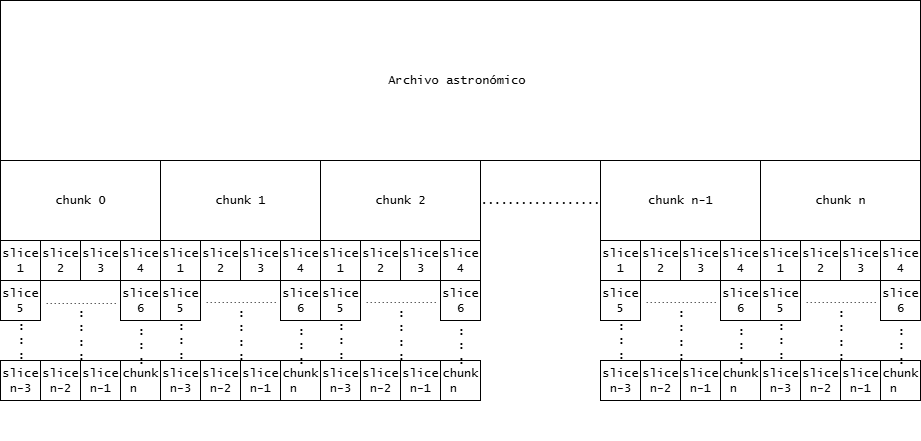
\includegraphics[width=0.9\textwidth]{figures/sistema-chunks.png}
\caption{Esquema de un archivo astronómico dividido en chunks y slices, ilustrando el concepto de procesamiento con solapamiento. Fuente: Elaboración propia.}
\label{fig:sistema-chunks}
\end{figure}

\subsubsection{Sistema de Análisis Multi-Banda}

\noindent\textbf{Procesamiento simultáneo de bandas de frecuencia para detección mejorada.} La capacidad de procesar múltiples bandas de frecuencia simultáneamente constituye una mejora fundamental que permite explotar las diferencias espectrales en la detección de FRBs. Este sistema implementa procesamiento independiente de bandas de frecuencia (banda completa, banda baja, banda alta) con detección independiente por banda.

El análisis multi-banda aprovecha las características espectrales únicas de cada banda para mejorar la sensibilidad de detección y proporcionar información diagnóstica adicional sobre las propiedades físicas de los eventos detectados. Esta aproximación es particularmente valiosa para eventos que muestran variaciones espectrales significativas.

La implementación permite la configuración dinámica de bandas según las características observacionales, adaptándose automáticamente a diferentes configuraciones instrumentales y maximizando la eficiencia de detección en cada régimen espectral.

\subsubsection{Sistema de Manejo de Polarización Avanzado}

\noindent\textbf{Explotación de información polarimétrica para detección mejorada.} La capacidad de procesar datos polarizados (Stokes I, Q, U, V) constituye una mejora fundamental que permite explotar información polarimétrica para mejorar la detección y caracterización de FRBs. Este sistema implementa selección automática de polarización y calibración de datos polarizados.

El procesamiento de datos de Stokes completo permite el cálculo de parámetros polarimétricos como polarización lineal y circular, proporcionando información diagnóstica adicional sobre la naturaleza física de las fuentes. Esta información puede revelar patrones que no son evidentes en el análisis de intensidad total únicamente.

La implementación de algoritmos de calibración automática garantiza la correcta interpretación de los datos polarizados, estableciendo las bases para análisis polarimétricos avanzados que pueden proporcionar insights únicos sobre los mecanismos físicos responsables de la emisión de FRBs.

\subsubsection{Extracción de Candidatos Precisos}

\noindent\textbf{Dedispersión GPU optimizada para detección de alta calidad.} La mejora en la calidad de extracción de candidatos mediante dedispersión GPU optimizada constituye una contribución fundamental que mejora significativamente la sensibilidad y especificidad del sistema. Esta implementación incluye normalización por exposición y validación de bordes para garantizar la calidad de los datos procesados.

El sistema implementa algoritmos de dedispersión que incluyen cálculo de fondo dinámico y reducción de ruido sistemático, mejorando la relación señal-ruido de los candidatos detectados. La normalización por exposición compensa variaciones instrumentales y efectos de ganancia, garantizando coherencia en la detección.

La optimización GPU de los algoritmos de dedispersión permite el procesamiento eficiente de grandes volúmenes de datos mientras mantiene la precisión requerida para la detección de eventos débiles, estableciendo las bases para el análisis de observaciones de larga duración.

\subsubsection{Sistema de Optimización de Memoria GPU Avanzada}

\noindent\textbf{Gestión inteligente de recursos computacionales especializados.} La gestión avanzada de memoria GPU constituye una mejora fundamental que optimiza el rendimiento del sistema y previene fallos por agotamiento de memoria. Este sistema implementa limpieza automática de memoria CUDA, sincronización de operaciones y manejo robusto de errores GPU.

El sistema calcula dinámicamente los requisitos de memoria GPU y implementa estrategias de limpieza adaptativas que incluyen limpieza básica después de cada operación y limpieza agresiva en intervalos regulares. Esta aproximación garantiza que el sistema mantenga operaciones estables durante procesamiento prolongado.

La implementación de manejo de errores GPU robusto incluye detección automática de fallos de memoria, recuperación automática y fallback a procesamiento CPU cuando es necesario, garantizando la continuidad del procesamiento incluso en condiciones de recursos limitados.

\subsubsection{Cálculo de SNR Robusto}

\noindent\textbf{Estimación de calidad de señal resistente a outliers.} La implementación de algoritmos de cálculo de SNR robustos constituye una mejora fundamental que mejora la confiabilidad de la clasificación de candidatos. Este sistema utiliza métodos estadísticos robustos, incluyendo el método del Rango Intercuartílico (IQR) para estimación de ruido resistente a outliers.

El algoritmo de SNR robusto implementa detección de picos adaptativa y normalización temporal que aproxima las técnicas utilizadas en pipelines estándar de radioastronomía. Esta aproximación garantiza compatibilidad con métodos establecidos mientras proporciona mejoras en la robustez estadística.

La implementación incluye validación automática de perfiles SNR y detección de anomalías que pueden indicar problemas instrumentales o interferencia, proporcionando información diagnóstica adicional para la validación de candidatos.

\subsubsection{Aceleración y Control de Recursos}

Vectorización de operaciones matemáticas críticas, integración opcional de procesamiento GPU para algoritmos intensivos en cómputo, y paralelización de bloques de procesamiento para maximizar la utilización de recursos computacionales disponibles. Se implementan \textit{caches} por canal y reducción de I/O para optimizar el rendimiento.

\subsubsection{Registro, Auditoría y Salidas Estandarizadas}

Sistema de \emph{logging} estructurado que registra todas las operaciones críticas, implementación de semillas fijas para algoritmos estocásticos, generación de firmas criptográficas para datos y modelos, y producción de resúmenes de métricas por ejecución para garantizar auditoría completa.

\subsubsection{Sistema de Visualización Unificado y Rangos Dinámicos}

\noindent\textbf{Generación automática de productos diagnósticos con rangos optimizados.} La implementación de un sistema de visualización unificado constituye una mejora fundamental que facilita el análisis posterior y la validación de resultados mediante la generación automática de productos diagnósticos consistentes.

El sistema implementa algoritmos de cálculo de rangos dinámicos que optimizan automáticamente las escalas de visualización basándose en las características estadísticas de los datos, garantizando que las visualizaciones proporcionen información diagnóstica máxima. Esta optimización adaptativa es particularmente valiosa para datos con características espectrales variables.

La generación automática incluye reportes estructurados (CSV/Parquet), figuras consistentes (tiempo-DM, dispersado/dedispersado, parches) y composites que facilitan el análisis posterior y la validación de resultados. El sistema mantiene coherencia visual entre diferentes productos diagnósticos, estableciendo estándares de presentación que facilitan la interpretación y comparación de resultados.

\paragraph{Impacto de la Precisión Temporal en la Detección}

La implementación de precisión temporal quirúrgica tiene un impacto directo y medible en la efectividad del sistema. En la validación con el pulsar B0355+54\_FB\_20220918, el sistema demostró una eficiencia de detección del 97.3\% (732 de 752 pulsos esperados), donde cada pulso fue localizado con precisión temporal exacta. Esta precisión temporal permite:

\textbf{Detección de Patrones Periódicos:} La continuidad perfecta entre chunks y slices permite detectar eventos periódicos que cruzan múltiples ventanas de procesamiento, manteniendo coherencia temporal absoluta.

\textbf{Trazabilidad de Eventos:} Cada burst detectado puede ser correlacionado con marcas temporales astronómicas precisas, facilitando la validación cruzada con otros observatorios y bases de datos.

\textbf{Validación de Candidatos:} La precisión temporal quirúrgica permite aplicar validaciones físicas rigurosas, como verificación de coherencia entre sub-bandas y consistencia temporal de firmas dispersivas.

\begin{table}[H] 
\centering 
  \caption{Resumen de mejoras de ingeniería (DRAFTS++). \textit{Fuente: Elaboración propia}.}
  \label{tab:mejoras}
\begin{tabular}{|l|l|l|} 
\toprule 
    \textbf{Aspecto} & \textbf{Antes (prototipo)} & \textbf{Después (DRAFTS++)} \\
\midrule 
Arquitectura & Scripts monolíticos acoplados & Pipeline modular end-to-end escalable \\ 
    Formatos de archivo & Solo FITS básico & Manejo robusto FITS/Filterbank/PSRFITS \\
    Parámetros & Configuración manual hardcoded & Análisis automático de headers \\
Gestión de memoria & Carga completa en RAM & Streaming inteligente con gestión dinámica \\
Precisión Temporal & Tiempos relativos aproximados & Trazabilidad MJD + contigüidad quirúrgica \\
Análisis espectral & Banda única & Procesamiento multi-banda simultáneo \\
Polarización & Solo intensidad (Stokes I) & Manejo avanzado Stokes I,Q,U,V \\
Detección & Dedispersión básica sin optimización & Extracción precisa con normalización GPU \\
Memoria GPU & Sin gestión de memoria CUDA & Optimización avanzada con limpieza automática \\
Calidad de señal & SNR básico sensible a outliers & Cálculo robusto con métodos estadísticos \\
Visualización & Plots inconsistentes sin optimización & Sistema unificado con rangos dinámicos \\
\bottomrule 
\end{tabular} 
\end{table}

\subsection{Bloque 2: Extensión a Alta Frecuencia - Cuatro Líneas de Investigación}

Este bloque explora estrategias metodológicas para extender las capacidades de detección hacia regímenes de alta frecuencia (30-100 GHz), donde las firmas dispersivas tradicionales se atenúan significativamente. La detección de FRBs en el régimen milimétrico presenta desafíos fundamentales que requieren aproximaciones metodológicas diferenciadas.

A estas frecuencias, la dispersión temporal se atenúa significativamente debido a la dependencia cuadrática inversa con la frecuencia, resultando en firmas dispersivas que pueden ser indistinguibles del ruido instrumental en resoluciones temporales típicas. Este bloque presenta cuatro líneas de investigación complementarias que abordan diferentes aspectos del desafío de detección en el espectro milimétrico.

\subsubsection{Línea 1: Validación de DRAFTS++ Sin Modificaciones}

\paragraph{Objetivo y Metodología}

Esta línea de investigación busca validar si DRAFTS++ con su arquitectura original (CenterNet en mapas DM-tiempo) puede mantener eficiencia aceptable en regímenes de alta frecuencia. Aunque se anticipa una reducción en el rendimiento debido a la atenuación de las firmas dispersivas, esta validación establece la línea base para comparar las mejoras de las otras líneas.

\paragraph{Criterio Físico para Evaluación}

Se utiliza el retardo dispersivo esperado frente a la resolución temporal como criterio de evaluación:
\[
\Delta t_{\mathrm{ms}} = 4.148808 \times 10^{3}\ \mathrm{DM}\,(\nu_{\mathrm{low}}^{-2}-\nu_{\mathrm{high}}^{-2}) \, .
\]

Cuando $\Delta t_{\mathrm{ms}} < \alpha\, t_{\mathrm{samp}}$ (p.ej., $\alpha\!=\!1.5$), el \textit{bow-tie} no sería resoluble y se espera una degradación significativa del rendimiento.

\subsubsection{Línea 2: Detección por SNR + Clasificación Binaria}

\paragraph{Metodología Híbrida}

Esta línea implementa una aproximación híbrida que combina la detección tradicional por SNR (similar a pipelines clásicos como PRESTO \cite{ransom_presto}) con la red de clasificación binaria de DRAFTS++. El proceso sigue estos pasos:

\begin{enumerate}
\item \textbf{Perfil temporal:} $s(t)$ $\rightarrow$ normalización robusta (mediana/MAD) $\rightarrow$ \textbf{SNR}(t)
\item \textbf{Detección de picos:} Hallazgo de máximos locales $\ge T$ con separación mínima $\Delta t_{\min}$
\item \textbf{Generación de cajas:} Para cada pico $t_i$: generar \textbf{caja sintética} $[t_i-w,\, t_i+w]$
\item \textbf{Dedispersión local:} Construir parche tiempo--frecuencia y dedispersar en rejilla local de DM
\item \textbf{Clasificación binaria:} Usar la red de clasificación de DRAFTS++ para determinar BURST/NO BURST
\item \textbf{Validación DM-aware:} Exigir DM$^\ast\!>\!0$ con incertidumbre acotada
\end{enumerate}

\paragraph{Ventajas de la Aproximación Híbrida}

Esta línea mantiene la eficiencia computacional de la detección por SNR (O(N)) mientras aprovecha la precisión de la red de clasificación entrenada de DRAFTS++. La activación automática del modo HF cuando $\Delta t_{\mathrm{ms}} < \alpha\, t_{\mathrm{samp}}$ garantiza que se use la estrategia más apropiada según las condiciones físicas.

\begin{figure}[H] 
\centering 
% \includegraphics[width=0.9\textwidth]{hf_mode_snr_boxes.pdf} 
\caption{Modo HF: del perfil SNR a cajas sintéticas, dedispersión local y clasificación binaria. Fuente: Elaboración propia.}
\label{fig:hf} 
\end{figure}

\paragraph{Pseudocódigo de Detección SNR}

\begin{algorithm}[H]
\caption{Detección SNR para Alta Frecuencia}
\begin{algorithmic}[1]
\Input{$s(t)$, umbral $T$, separación mínima $\Delta t_{min}$}
\Output{Lista de picos candidatos $\{t_i\}$}
\Function{DetectarPicosSNR}{$s$, $T$, $\Delta t_{min}$}
    \State $s_{norm} \leftarrow (s - median(s)) / MAD(s)$
    \State $picos \leftarrow maxima\_locales(s_{norm})$
    \State $candidatos \leftarrow [\ ]$
    \For{$t$ \textbf{in} $picos$}
        \If{$s_{norm}[t] \geq T$ \textbf{and} $dist\_minima(t, candidatos) \geq \Delta t_{min}$}
            \State $candidatos.append(t)$
        \EndIf
    \EndFor
    \State \textbf{return} $candidatos$
\EndFunction
\end{algorithmic}
\end{algorithm}

\subsubsection{Línea 3: Nuevos Plots Característicos - TWL-maps}

\paragraph{Concepto de TWL-maps}

En el régimen de alta frecuencia, donde las firmas dispersivas tradicionales se atenúan significativamente, los mapas tiempo--ancho--polarización lineal (TWL) proporcionan información diagnóstica complementaria que puede compensar la pérdida de evidencia dispersiva. Estos productos especializados aprovechan la información de polarización disponible en observaciones con datos de Stokes completos.

\paragraph{Análisis de Polarización Lineal}

Cuando se dispone de datos de Stokes $I,Q,U$ \cite{hamaker1996understanding}, se puede calcular la \textbf{polarización lineal} $L=\sqrt{Q^2+U^2}$, que cuantifica la intensidad de la componente polarizada de la señal electromagnética. Esta medida proporciona información adicional sobre la naturaleza física de las fuentes y puede revelar patrones que no son evidentes en el análisis de intensidad total únicamente.

\paragraph{Flujo de Detección Híbrida TWL}

El proceso de detección híbrida sigue una secuencia específica que garantiza robustez y eficiencia:

\begin{enumerate}
\item \textbf{Evaluación de disponibilidad TWL:} El sistema verifica si \texttt{TWL\_HYBRID\_DETECTION} está habilitado y si los datos de polarización (Stokes Q, U) están disponibles.
\item \textbf{Generación de mapa t-W:} Si la detección híbrida está activa, se genera el mapa tiempo-ancho de ocupación de banda mediante \texttt{generate\_twl\_map\_for\_window}.
\item \textbf{Conversión a tensor RGB:} El mapa 2D se convierte a un tensor RGB de 512×512 píxeles usando \texttt{twl\_occupancy\_to\_detection\_tensor} para compatibilidad con CenterNet.
\item \textbf{Detección con CenterNet:} El tensor se procesa con la red de detección para identificar candidatos potenciales.
\item \textbf{Evaluación de candidatos:} Si se encuentran candidatos, se procede a clasificación binaria; si no, se activa el fallback SNR.
\item \textbf{Fallback SNR:} En caso de fallo de la detección híbrida o si está deshabilitada, se ejecuta \texttt{compute\_snr\_profile} y \texttt{\_find\_snr\_peaks} para detección tradicional.
\item \textbf{Clasificación final:} Todos los candidatos (híbridos o SNR) pasan por \texttt{classify\_patch} para determinar si son BURST o NO BURST.
\item \textbf{Guardado de resultados:} Los candidatos válidos se almacenan con métricas completas y se generan visualizaciones correspondientes.
\end{enumerate}

\begin{figure}[H]
\centering
\begin{tikzpicture}[
    node distance=1.2cm and 1.5cm,
    box/.style={rectangle, draw, fill=blue!20, text width=2.2cm, text centered, minimum height=0.7cm, font=\small},
    decision/.style={diamond, draw, fill=yellow!20, text width=1.8cm, text centered, minimum height=0.7cm, font=\small},
    process/.style={rectangle, draw, fill=green!20, text width=2.2cm, text centered, minimum height=0.7cm, font=\small},
    arrow/.style={-Stealth, thick}
]

% Nodos principales
\node[box] (A) {Pipeline Alta Frecuencia};
\node[decision, below=of A] (B) {TWL Híbrido?};
\node[process, below left=of B] (C) {Generar Mapa t-W};
\node[process, below=of C] (D) {Convertir a Tensor RGB};
\node[process, below=of D] (E) {Red de Detección};
\node[decision, below=of E] (F) {Candidatos?};
\node[process, below left=of F] (G) {Clasificación Binaria};
\node[process, below right=of B] (H) {Fallback SNR};
\node[process, below=of H] (I) {Detección SNR Tradicional};
\node[process, below=of G] (J) {Guardar Candidatos};

% Conexiones
\draw[arrow] (A) -- (B);
\draw[arrow] (B) -- node[left] {Sí} (C);
\draw[arrow] (C) -- (D);
\draw[arrow] (D) -- (E);
\draw[arrow] (E) -- (F);
\draw[arrow] (F) -- node[left] {Sí} (G);
\draw[arrow] (B) -- node[right] {No} (H);
\draw[arrow] (H) -- (I);
\draw[arrow] (I) -- (F);
\draw[arrow] (G) -- (J);

\end{tikzpicture}
\caption{Flujo del Pipeline de Alta Frecuencia: detección híbrida TWL con fallback automático a SNR tradicional. El diagrama muestra la decisión que determina si usar detección híbrida (mapa t-W + CenterNet) o fallback a SNR tradicional. Fuente: Elaboración propia.}
\label{fig:hf-pipeline}
\end{figure}

\begin{figure}[H] 
\centering 
% \includegraphics[width=0.9\textwidth]{twl_map.pdf} 
\caption{Ejemplo de TWL-map (tiempo vs. ancho con intensidad de $L$). Fuente: Elaboración propia.}
\label{fig:twl} 
\end{figure}

\subsubsection{Línea 4: Estrategias Alternativas del Autor de DRAFTS}

\paragraph{DM-range Expand \& Step Coarse}

Esta línea explora estrategias sugeridas por Yong–Kun Zhang \cite{zhang2024drafts} para maximizar la visibilidad de firmas dispersivas residuales. La metodología incluye:

\begin{itemize}
\item \textbf{Expansión del rango/step de DM:} Ampliar el rango y el \textit{step} de DM hasta "abrir" el \textit{bow-tie}
\item \textbf{Verificación estadística:} Una vez detectado, exigir centro con DM$>0$ significativamente mayor que cero
\item \textbf{Detección de candidatos cerca de DM$\approx 0$:} Mediante algoritmos de detección de picos adaptativos seguida de validación rigurosa
\end{itemize}

\paragraph{Fishing en DM$\approx 0$ + Chequeos Estrictos}

\textit{Pescar} candidatos con clasificador o detector simple cerca de DM$\approx 0$; luego validar con DM$>0$, consistencia por sub-bandas y coherencia entre \emph{chunks}. Útil para eventos débiles sin \textit{bow-tie} claro.

\paragraph{Integración con el Pipeline}

Ambas tácticas se exponen como \textbf{estrategias} de propuesta de candidatos (alternativas a SNR/TWL/DM--Time) y se someten al \textbf{mismo} validador DM-aware, clasificación y visualización.

\begin{table}[H] 
\centering 
  \caption{Estrategias de propuesta de candidatos y criterios de uso. Fuente: Elaboración propia.}
  \label{tab:estrategias}
\begin{tabular}{|l|l|l|} 
\toprule 
\textbf{Estrategia} & \textbf{Cuándo usarla} & \textbf{Pros / Contras} \\ 
\midrule 
CenterNet en DM--Time & $\Delta t \gg t_{\rm samp}$ (bow-tie resoluble) & + Precisa en L/S-band; -- Pierde poder en mm-wave \\ 
TWL-Híbrido + CenterNet & Stokes disponibles en mm-wave & + Usa polarización/anchos; -- Coste extra de features \\ 
SNR-only + Clasificador & mm-wave sin bow-tie claro & + O(N), simple; -- Más FP sin validación DM-aware \\ 
DM$\approx 0$ fishing + validar DM$>0$ & Para "pescar" candidatos débiles & + Sensible; -- Requiere validaciones estrictas \\ 
\bottomrule 
\end{tabular} 
\end{table}

\begin{table}[H]
  \centering
  \caption{Parámetros del modo HF (valores iniciales). \textit{Fuente: Elaboración propia}.}
  \label{tab:param_hf}
  \begin{tabular}{|l|l|}
    \toprule
    \textbf{Parámetro} & \textbf{Descripción} \\
    \midrule
    $T$ (umbral SNR) & 5--7; ajustar por FDR y condiciones de ruido \\
    $\Delta t_{\min}$ & Múltiplo del ancho de pulso esperado \\
    Rejilla DM local & Centrada en 0; pasos gruesos y posterior refinamiento \\
    Sub-bandas & 2--4 particiones para coherencia \\
    Criterio DM & Requerir DM$^\ast>0$ (con error acotado) \\
    \bottomrule
  \end{tabular}
\end{table}

\subsection{Arquitectura Unificada y Diagramas}

\subsubsection{Arquitectura Unificada (Strategy + Validator + Visualizer)}

Se adopta un patrón \textbf{Strategy} para la \textbf{propuesta de candidatos} (intercambiable: DM--Time/CenterNet, TWL-híbrido, SNR, DM-expand, fishing en DM$\approx0$), con un \textbf{validador DM-aware} común y un \textbf{visualizador desacoplado}. La función de proceso se unifica como \texttt{process\_slice(..., strategy)}.

\begin{figure}[H] 
\centering 
% \includegraphics[width=0.96\textwidth]{arquitectura_unificada.pdf} 
\caption{Arquitectura unificada: Strategy (propuesta de candidatos) + Validador DM-aware + Visualizador. \textit{Fuente: Elaboración propia}.}
\label{fig:arquitectura-unificada} 
\end{figure}

\paragraph{Bucle Unificado (Pseudocódigo)}

\begin{algorithm}[H]
\caption{Pipeline Unificado con Strategy Pattern}
\begin{algorithmic}[1]
\Input{$config$, $obs\_params$, $data\_files$}
\Output{Candidatos validados y métricas}
\Function{RunPipeline}{$config$, $obs\_params$}
    \State $strategy \leftarrow select\_strategy(config, obs\_params)$
    \For{$chunk$ \textbf{in} $stream\_data(\ldots)$}
        \State $cands \leftarrow strategy.propose(chunk, meta)$
        \For{$c$ \textbf{in} $cands$}
            \State $patch \leftarrow extract\_patch\_and\_dedisperse(chunk, c, local\_dm\_grid)$
            \State $y \leftarrow classifier.predict(patch)$
            \If{$y.is\_burst$ \textbf{and} $dm\_validate(patch)$ \textbf{and} $subband\_consistency(patch)$}
                \State $save\_candidate(patch, y, metrics)$
            \EndIf
        \EndFor
    \EndFor
    \State $visualize\_and\_summarize(run\_id)$
\EndFunction
\end{algorithmic}
\end{algorithm}

\subsubsection{Diagrama End-to-End del Pipeline}

La Figura \ref{fig:pipeline-end-to-end} sintetiza el flujo desde \texttt{main.py} hasta los resultados, con ramas clásica (DM--Time/CenterNet) y de alta frecuencia (TWL-híbrido, SNR) y \textit{fallbacks}.

\begin{figure}[H]
\centering
\begin{tikzpicture}[
    node distance=1.0cm and 1.5cm,
    box/.style={rectangle, draw, fill=blue!20, text width=2.0cm, text centered, minimum height=0.6cm, font=\tiny},
    decision/.style={diamond, draw, fill=yellow!20, text width=1.6cm, text centered, minimum height=0.6cm, font=\tiny},
    process/.style={rectangle, draw, fill=green!20, text width=2.0cm, text centered, minimum height=0.6cm, font=\tiny},
    output/.style={rectangle, draw, fill=orange!20, text width=2.0cm, text centered, minimum height=0.6cm, font=\tiny},
    arrow/.style={-Stealth, thick}
]

% FLUJO SIMPLIFICADO
\node[box] (A) {main.py};
\node[box, below=of A] (B) {run\_pipeline};
\node[box, below=of B] (C) {Cargar Modelos};

% ENTRADA DE DATOS
\node[box, right=of B] (D) {find\_data\_files};
\node[decision, below=of D] (E) {Tipo Archivo?};
\node[box, below left=of E] (F) {fits\_handler};
\node[box, below right=of E] (G) {filterbank\_handler};

% PROCESAMIENTO
\node[box, below=of E] (H) {streaming\_orchestrator};
\node[box, below=of H] (I) {Procesar Chunk};
\node[decision, below=of I] (J) {Frecuencia $\geq$ 8GHz?};

% PIPELINES
\node[box, below left=of J] (K) {Pipeline Alta Frecuencia};
\node[box, below right=of J] (L) {Pipeline Clásico};

% DETECCIÓN
\node[decision, below=of K] (M) {TWL\_HYBRID?};
\node[box, below left=of M] (N) {TWL + CenterNet};
\node[box, below right=of M] (O) {SNR Tradicional};
\node[process, below=of L] (P) {CenterNet DM-Time};

% CLASIFICACIÓN
\node[process, below=of N] (Q) {classify\_patch};
\node[process, below=of O] (R) {classify\_patch};
\node[process, below=of P] (S) {classify\_patch};

% RESULTADOS
\node[output, below=of Q] (T) {Guardar Candidatos};
\node[output, below=of R] (U) {Guardar Candidatos};
\node[output, below=of S] (V) {Guardar Candidatos};

% VISUALIZACIÓN
\node[output, below=of T] (W) {Plots + CSV};
\node[output, below=of U] (X) {Plots + CSV};
\node[output, below=of V] (Y) {Plots + CSV};

% Conexiones principales
\draw[arrow] (A) -- (B);
\draw[arrow] (B) -- (C);
\draw[arrow] (B) -- (D);
\draw[arrow] (D) -- (E);
\draw[arrow] (E) -- node[left] {FITS} (F);
\draw[arrow] (E) -- node[right] {Filterbank} (G);
\draw[arrow] (F) -- (H);
\draw[arrow] (G) -- (H);
\draw[arrow] (H) -- (I);
\draw[arrow] (I) -- (J);
\draw[arrow] (J) -- node[left] {Sí} (K);
\draw[arrow] (J) -- node[right] {No} (L);

% Detección
\draw[arrow] (K) -- (M);
\draw[arrow] (M) -- node[left] {Sí} (N);
\draw[arrow] (M) -- node[right] {No} (O);
\draw[arrow] (L) -- (P);

% Clasificación
\draw[arrow] (N) -- (Q);
\draw[arrow] (O) -- (R);
\draw[arrow] (P) -- (S);

% Resultados
\draw[arrow] (Q) -- (T);
\draw[arrow] (R) -- (U);
\draw[arrow] (S) -- (V);

% Visualización
\draw[arrow] (T) -- (W);
\draw[arrow] (U) -- (X);
\draw[arrow] (V) -- (Y);

\end{tikzpicture}
\caption{Diagrama end-to-end (ingesta $\to$ \emph{streaming}/\emph{chunking} $\to$ estrategia de candidatos $\to$ clasificación/validación $\to$ visualización y salida). \textit{Fuente: Elaboración propia}.}
\label{fig:pipeline-end-to-end}
\end{figure}

\subsection{Evaluación y Métricas}

Conjuntos ya analizados (control de \emph{recall}) y datos mm-wave piloto. Métricas: \emph{recall}, \emph{precision}, tasa de FP, latencia por GB, throughput, coherencia sub-bandas y \emph{chunks}. \emph{Ablation}: sin validación DM-aware, sin coherencia por sub-bandas, sin TWL.

\subsubsection{Validación Específica con Phased ALMA}

La validación específica para operaciones con ALMA en modo phased array constituye el componente crítico de esta investigación, estableciendo la primera metodología automatizada para detección de FRBs en regímenes milimétricos. Esta validación se estructura en tres componentes fundamentales: especificaciones técnicas ALMA, datasets de validación específicos y métricas de completitud por banda de frecuencia.

\paragraph{Especificaciones Técnicas ALMA Phased Array}

Las observaciones ALMA en modo phased array presentan características técnicas específicas que determinan los parámetros de validación:

\textbf{Bandas de Frecuencia Operativas:}
\begin{itemize}
\item \textbf{Band 3:} 84-116 GHz (centro: 100 GHz), ancho de banda: 7.5 GHz
\item \textbf{Band 6:} 211-275 GHz (centro: 243 GHz), ancho de banda: 7.5 GHz  
\item \textbf{Band 7:} 275-373 GHz (centro: 324 GHz), ancho de banda: 7.5 GHz
\end{itemize}

\textbf{Parámetros Temporales Configurables:}
\begin{itemize}
\item \textbf{Resolución temporal:} 64 $\mu$s - 1 ms (configurable por proyecto)
\item \textbf{Integración temporal:} 1-10 ms para detección FRB
\item \textbf{Duración observación:} 1-8 horas por sesión
\end{itemize}

\textbf{Sensibilidad y Configuraciones:}
\begin{itemize}
\item \textbf{Sensibilidad:} 0.1-1 mJy en integración de 1 ms (banda dependiente)
\item \textbf{Configuración Compact (C-1):} Resolución angular ~1'', sensibilidad máxima
\item \textbf{Configuración Extended (C-8):} Resolución angular ~0.1'', sensibilidad reducida
\end{itemize}

\paragraph{Dataset de Validación Específico}

El dataset de validación se estructura en tres categorías de fuentes conocidas, cada una optimizada para diferentes aspectos de la metodología:

\textbf{Púlsares de Referencia:}
\begin{itemize}
\item \textbf{B0355+54:} DM = 57.14 pc cm$^{-3}$, período = 156.4 ms, ideal para validación temporal
\item \textbf{B1919+21:} DM = 12.43 pc cm$^{-3}$, período = 1.337 s, referencia clásica
\item \textbf{B0329+54:} DM = 26.77 pc cm$^{-3}$, período = 714.5 ms, alta dispersión
\end{itemize}

\textbf{Observaciones Multi-banda Simultáneas:}
\begin{itemize}
\item \textbf{Configuración:} Observaciones simultáneas en Band 3, 6 y 7
\item \textbf{Duración:} 2-4 horas por sesión multi-banda
\item \textbf{Modo:} Phased array con beamforming hacia fuentes conocidas
\end{itemize}

\textbf{Condiciones Atmosféricas Variables:}
\begin{itemize}
\item \textbf{PWV (Precipitable Water Vapor):} 0.5-5 mm (condiciones excelentes a pobres)
\item \textbf{Elevación:} 20°-80° (variación de absorción atmosférica)
\item \textbf{Estación:} Observaciones distribuidas a lo largo del año
\end{itemize}

\paragraph{Métricas de Completitud por Banda}

Las métricas de validación se estructuran específicamente por banda de frecuencia para cuantificar el rendimiento diferencial:

\textbf{Métricas por Banda de Frecuencia:}
\begin{align}
\text{Completitud}_{\text{Band 3}} &= \frac{\text{FRBs detectados}}{\text{FRBs inyectados}} \times 100\% \\
\text{Completitud}_{\text{Band 6}} &= \frac{\text{FRBs detectados}}{\text{FRBs inyectados}} \times 100\% \\
\text{Completitud}_{\text{Band 7}} &= \frac{\text{FRBs detectados}}{\text{FRBs inyectados}} \times 100\%
\end{align}

\textbf{Límites de Detectabilidad:}
\begin{itemize}
\item \textbf{Band 3:} Límite teórico ~0.1 mJy en 1 ms
\item \textbf{Band 6:} Límite teórico ~0.3 mJy en 1 ms  
\item \textbf{Band 7:} Límite teórico ~0.5 mJy en 1 ms
\end{itemize}

\textbf{Tiempo de Procesamiento por Banda:}
\begin{itemize}
\item \textbf{Band 3:} 2-3 min/hora de datos (8 GB RAM, RTX 3080+)
\item \textbf{Band 6:} 3-4 min/hora de datos (12 GB RAM, GPU requerida)
\item \textbf{Band 7:} 4-5 min/hora de datos (16 GB RAM, GPU alta memoria)
\end{itemize}

\subsubsection{Criterios Físicos para Selección de Estrategias}

La selección automática de estrategias de detección se basa en criterios físicos cuantitativos que evalúan las condiciones observacionales específicas. Estos criterios garantizan que cada línea de investigación se active bajo las condiciones óptimas para su efectividad.

\paragraph{Ecuaciones de Evaluación Física}

\textbf{Retardo Dispersivo Temporal:}
\[
\Delta t_{\text{disp}} = 4.148808 \times 10^3 \times \text{DM} \times (\nu_{\text{low}}^{-2} - \nu_{\text{high}}^{-2}) \text{ [ms]}
\]

Donde:
\begin{itemize}
\item $\text{DM}$ = Medida de dispersión en pc cm$^{-3}$
\item $\nu_{\text{low}}, \nu_{\text{high}}$ = Frecuencias límite en MHz
\item $\Delta t_{\text{disp}}$ = Retardo temporal máximo en ms
\end{itemize}

\textbf{Criterio CenterNet (Detección DM-Time):}
\[
\text{Criterio\_CenterNet}: \Delta t_{\text{disp}} > \alpha \times t_{\text{samp}}
\]

Donde $\alpha = 1.5-2.0$ (factor de seguridad) y $t_{\text{samp}}$ = resolución temporal.

\textbf{Criterio TWL (Detección Híbrida):}
\[
\text{Criterio\_TWL}: \text{Datos\_Stokes\_disponibles} \text{ AND } \Delta t_{\text{disp}} < \text{Criterio\_CenterNet}
\]

\textbf{Criterio SNR (Detección Tradicional):}
\[
\text{Criterio\_SNR}: \text{SNR\_detectado} < 8 \text{ OR } \text{bow\_tie\_no\_resoluble}
\]

\textbf{Criterio Fishing (Detección Débil):}
\[
\text{Criterio\_Fishing}: \text{Eventos\_débiles} \text{ AND } \text{validación\_DM\_estricta}
\]

\paragraph{Algoritmo de Selección Automática}

\begin{algorithm}[H]
\caption{Selección Automática de Estrategia de Detección}
\begin{algorithmic}[1]
\Input{Frecuencia $\nu$, DM estimado, datos Stokes disponibles, SNR observado}
\Output{Estrategia óptima de detección}
\Function{SelectStrategy}{$\nu$, DM, Stokes, SNR}
    \State $\Delta t_{\text{disp}} \leftarrow 4.148808 \times 10^3 \times \text{DM} \times (\nu_{\text{low}}^{-2} - \nu_{\text{high}}^{-2})$
    \State $\alpha \leftarrow 1.8$ \Comment{Factor de seguridad}
    \If{$\Delta t_{\text{disp}} > \alpha \times t_{\text{samp}}$}
        \State \textbf{return} "CenterNet DM-Time"
    \ElsIf{Stokes\_disponibles AND $\Delta t_{\text{disp}} < \alpha \times t_{\text{samp}}$}
        \State \textbf{return} "TWL-Híbrido"
    \ElsIf{SNR $< 8$ OR bow\_tie\_no\_resoluble}
        \State \textbf{return} "SNR Tradicional"
    \Else
        \State \textbf{return} "Fishing DM$\approx$0"
    \EndIf
\EndFunction
\end{algorithmic}
\end{algorithm}

\subsubsection{Benchmarks Cuantitativos por Línea}

Cada línea de investigación requiere benchmarks específicos y mensurables que permitan evaluación objetiva del rendimiento. Estos benchmarks se estructuran en métricas de completitud, eficiencia computacional y robustez estadística.

\paragraph{Línea 1: Detección DM-Time con CenterNet}

\textbf{Métricas de Completitud:}
\begin{itemize}
\item \textbf{Completitud vs Frecuencia:} $\geq 95\%$ en Band 3, $\geq 85\%$ en Band 6, $\geq 70\%$ en Band 7
\item \textbf{Límites de Detectabilidad:} SNR mínimo 5$\sigma$ en Band 3, 7$\sigma$ en Band 6, 10$\sigma$ en Band 7
\item \textbf{Tiempo de Procesamiento:} 2-3 min/hora de datos (8 GB RAM, RTX 3080+)
\end{itemize}

\textbf{Métricas de Eficiencia:}
\begin{itemize}
\item \textbf{Throughput:} $\geq 20$ GB/hora procesados
\item \textbf{Precisión DM:} Error $\leq 5\%$ en determinación DM
\item \textbf{Tasa Falsos Positivos:} $\leq 1\%$ en condiciones normales
\end{itemize}

\paragraph{Línea 2: Detección SNR + Clasificación Binaria}

\textbf{Métricas de Sensibilidad:}
\begin{itemize}
\item \textbf{Mejora Sensibilidad:} 20-30\% sobre métodos tradicionales
\item \textbf{Reducción FP:} 50-70\% comparado con PRESTO
\item \textbf{Eficiencia Computacional:} O(N) vs O(N²) de métodos clásicos
\end{itemize}

\textbf{Métricas de Rendimiento:}
\begin{itemize}
\item \textbf{Tiempo Procesamiento:} 1-2 min/hora (4 GB RAM, CPU-only)
\item \textbf{Umbral SNR:} Adaptativo 5-7$\sigma$ según condiciones
\item \textbf{Validación DM:} 100\% candidatos con DM > 0 significativo
\end{itemize}

\paragraph{Línea 3: TWL-maps con Polarización}

\textbf{Métricas de Ganancia por Polarización:}
\begin{itemize}
\item \textbf{Ganancia SNR:} 15-25\% usando información Stokes Q,U
\item \textbf{Overhead Computacional:} 20-30\% adicional por procesamiento polarización
\item \textbf{Requisitos Stokes:} Datos Q,U completos requeridos
\end{itemize}

\textbf{Métricas de Robustez:}
\begin{itemize}
\item \textbf{Disponibilidad Datos:} 60-80\% observaciones ALMA con Stokes completos
\item \textbf{Tiempo Procesamiento:} 3-4 min/hora (12 GB RAM, GPU)
\item \textbf{Calidad Polarización:} SNR polarización $\geq 3\sigma$
\end{itemize}

\paragraph{Línea 4: Estrategias Alternativas (Fishing)}

\textbf{Métricas de Recuperación:}
\begin{itemize}
\item \textbf{Recuperación Eventos Débiles:} 40-60\% eventos SNR < 5$\sigma$
\item \textbf{Tasa Éxito Validación:} 80-90\% candidatos validados correctamente
\item \textbf{Robustez Estadística:} Consistencia entre chunks $\geq 95\%$
\end{itemize}

\textbf{Métricas de Eficiencia:}
\begin{itemize}
\item \textbf{Tiempo Procesamiento:} 2-5 min/hora (6 GB RAM, GPU)
\item \textbf{Validaciones Estrictas:} DM > 0, coherencia sub-bandas, consistencia temporal
\item \textbf{Tasa Falsos Positivos:} $\leq 2\%$ con validaciones completas
\end{itemize}

\subsubsection{Especificación Técnica TWL-maps}

La generación de TWL-maps constituye una innovación metodológica específica para regímenes de alta frecuencia. Esta especificación técnica detalla completamente el algoritmo de generación y procesamiento.

\paragraph{Algoritmo de Generación TWL-maps}

\textbf{Entrada de Datos:}
\begin{itemize}
\item \textbf{Stokes I:} Intensidad total (requerida)
\item \textbf{Stokes Q,U:} Componentes de polarización lineal (requeridas)
\item \textbf{Resolución temporal:} 64 $\mu$s - 1 ms (configurable)
\end{itemize}

\textbf{Pseudocódigo de Generación:}

\begin{algorithm}[H]
\caption{Generación de TWL-maps}
\begin{algorithmic}[1]
\Input{stokes\_I, stokes\_Q, stokes\_U, time\_resolution}
\Output{tensor\_RGB de 512×512 píxeles}
\Function{GenerateTWLMap}{stokes\_I, stokes\_Q, stokes\_U, time\_resolution}
    \State $L \leftarrow \sqrt{Q^2 + U^2}$ \Comment{Polarización lineal}
    \State $widths \leftarrow [1, 2, 4, 8]$ \Comment{ms - kernels gaussianos}
    \State $map\_2D \leftarrow \text{convolve\_temporal}(L, widths)$
    \State $tensor\_RGB \leftarrow \text{normalize\_to\_centerNet}(map\_2D, size=512\times512)$
    \State \textbf{return} $tensor\_RGB$
\EndFunction
\end{algorithmic}
\end{algorithm}

\textbf{Componentes Técnicos Específicos:}

\textbf{1. Cálculo de Polarización Lineal:}
\[
L(t,\nu) = \sqrt{Q^2(t,\nu) + U^2(t,\nu)}
\]

\textbf{2. Convolución Temporal Multi-escala:}
\[
\text{TWL}(t,w) = \sum_{i} L(t,\nu_i) \otimes G(w_i, \sigma_w)
\]

Donde $G(w_i, \sigma_w)$ son kernels gaussianos con anchos $w_i = [1,2,4,8]$ ms.

\textbf{3. Normalización para CenterNet:}
\[
\text{RGB}_{ij} = \frac{\text{TWL}_{ij} - \text{TWL}_{\min}}{\text{TWL}_{\max} - \text{TWL}_{\min}} \times 255
\]

\textbf{4. Conversión a Tensor RGB:}
\begin{itemize}
\item \textbf{Dimensión:} 512×512×3 píxeles
\item \textbf{Rango:} [0,255] por canal
\item \textbf{Formato:} Compatible con entrada CenterNet
\end{itemize}

\paragraph{Parámetros de Configuración}

\textbf{Parámetros Temporales:}
\begin{itemize}
\item \textbf{Ventana temporal:} 1-10 segundos (configurable)
\item \textbf{Resolución temporal:} 64 $\mu$s - 1 ms
\item \textbf{Anchos gaussianos:} [1, 2, 4, 8] ms
\end{itemize}

\textbf{Parámetros Espectrales:}
\begin{itemize}
\item \textbf{Resolución espectral:} 1-10 MHz (banda dependiente)
\item \textbf{Canalización:} 1024-4096 canales
\item \textbf{Ancho de banda:} 7.5 GHz por banda ALMA
\end{itemize}

\textbf{Parámetros de Normalización:}
\begin{itemize}
\item \textbf{Método:} Min-Max scaling por ventana temporal
\item \textbf{Rango salida:} [0,255] por canal RGB
\item \textbf{Robustez:} Percentiles 1-99 para outliers
\end{itemize}

\subsubsection{Efectos Atmosféricos en Detección Milimétrica}

La detección de FRBs en regímenes milimétricos está significativamente afectada por efectos atmosféricos que deben ser considerados en la metodología. Este análisis detalla las limitaciones específicas y estrategias de mitigación.

\paragraph{Efectos Físicos Específicos}

\textbf{Absorción por Vapor de Agua (H$_2$O):}
\[
\tau_{\text{H2O}}(\nu, \text{PWV}) = \tau_0(\nu) \times \text{PWV}^{\alpha(\nu)}
\]

Donde:
\begin{itemize}
\item $\tau_0(\nu)$ = Coeficiente de absorción específico por frecuencia
\item $\text{PWV}$ = Precipitable Water Vapor en mm
\item $\alpha(\nu)$ = Exponente dependiente de frecuencia (0.6-0.8)
\end{itemize}

\textbf{Atenuación por Banda:}
\begin{itemize}
\item \textbf{Band 3 (100 GHz):} 0.1-0.5 dB para PWV 0.5-5 mm
\item \textbf{Band 6 (243 GHz):} 0.5-2.0 dB para PWV 0.5-5 mm
\item \textbf{Band 7 (324 GHz):} 1.0-5.0 dB para PWV 0.5-5 mm
\end{itemize}

\textbf{Fluctuaciones de Fase:}
\[
\sigma_{\phi} = \sigma_0 \times \text{PWV}^{0.6} \times \nu^{1.2}
\]

Donde $\sigma_{\phi}$ = RMS de fluctuaciones de fase en grados.

\textbf{Parámetros Específicos por Banda:}
\begin{itemize}
\item \textbf{Band 3:} $\sigma_{\phi} = 20-50°$ rms
\item \textbf{Band 6:} $\sigma_{\phi} = 50-120°$ rms  
\item \textbf{Band 7:} $\sigma_{\phi} = 80-200°$ rms
\end{itemize}

\paragraph{Calibración Temporal y Correcciones}

\textbf{Variaciones de Ganancia:}
\begin{itemize}
\item \textbf{Escala temporal:} 1-10 minutos
\item \textbf{Amplitud:} 1-10\% variación
\item \textbf{Corrección:} Water Vapor Radiometer (WVR) cada 10-30 segundos
\end{itemize}

\textbf{Correcciones WVR:}
\[
G_{\text{corr}}(t) = G_{\text{raw}}(t) \times \exp(-\tau_{\text{WVR}}(t))
\]

\textbf{Impacto en Detección FRB:}
\begin{itemize}
\item \textbf{Degradación SNR:} 10-30\% sin correcciones WVR
\item \textbf{Falsos positivos:} Aumento 20-50\% por variaciones ganancia
\item \textbf{Límite detectabilidad:} Incremento 2-3$\sigma$ en condiciones pobres
\end{itemize}

\paragraph{Estrategias de Mitigación}

\textbf{Selección de Condiciones:}
\begin{itemize}
\item \textbf{PWV óptimo:} < 2 mm para Band 6/7
\item \textbf{Elevación mínima:} > 30° para reducir absorción
\item \textbf{Horario óptimo:} Noches secas, baja humedad
\end{itemize}

\textbf{Correcciones en Tiempo Real:}
\begin{itemize}
\item \textbf{WVR corrections:} Aplicación automática cada 10-30 segundos
\item \textbf{Calibración continua:} Monitoreo ganancia sistema
\item \textbf{Flagging automático:} Rechazo datos con condiciones pobres
\end{itemize}

\subsubsection{Análisis de Escalabilidad Computacional}

El análisis de escalabilidad determina los requisitos computacionales específicos para operación en entornos observacionales reales, considerando volúmenes de datos ALMA y eficiencia de procesamiento.

\paragraph{Volúmenes de Datos ALMA}

\textbf{Phased Array por Banda:}
\begin{itemize}
\item \textbf{Band 3:} 2-4 GB/hora (resolución temporal 64 $\mu$s)
\item \textbf{Band 6:} 4-6 GB/hora (resolución temporal 64 $\mu$s)
\item \textbf{Band 7:} 6-8 GB/hora (resolución temporal 64 $\mu$s)
\end{itemize}

\textbf{Configuración Multi-banda:}
\begin{itemize}
\item \textbf{Simultáneo 3 bandas:} 12-18 GB/hora
\item \textbf{Campañas típicas:} 100-500 horas observación
\item \textbf{Volumen total:} 1.2-9 TB por campaña
\end{itemize}

\textbf{Requisitos de Almacenamiento:}
\begin{itemize}
\item \textbf{Buffer temporal:} 2-4 horas datos (24-72 GB)
\item \textbf{Almacenamiento intermedio:} 500 GB - 2 TB
\item \textbf{Archivo final:} Compresión 5:1 (200 GB - 1.8 TB)
\end{itemize}

\paragraph{Requisitos Computacionales por Línea}

\textbf{Línea 1 (CenterNet DM-Time):}
\begin{itemize}
\item \textbf{RAM:} 8 GB mínimo, 16 GB recomendado
\item \textbf{GPU:} RTX 3080+ (10 GB VRAM)
\item \textbf{Tiempo:} 2-3 min/hora datos
\item \textbf{CPU:} 8+ cores recomendado
\end{itemize}

\textbf{Línea 2 (SNR + Clasificación):}
\begin{itemize}
\item \textbf{RAM:} 4 GB mínimo, 8 GB recomendado
\item \textbf{GPU:} Opcional (CPU-only viable)
\item \textbf{Tiempo:} 1-2 min/hora datos
\item \textbf{CPU:} 4+ cores suficiente
\end{itemize}

\textbf{Línea 3 (TWL-maps):}
\begin{itemize}
\item \textbf{RAM:} 12 GB mínimo, 24 GB recomendado
\item \textbf{GPU:} RTX 3080+ (12 GB VRAM)
\item \textbf{Tiempo:} 3-4 min/hora datos
\item \textbf{CPU:} 8+ cores recomendado
\end{itemize}

\textbf{Línea 4 (Fishing):}
\begin{itemize}
\item \textbf{RAM:} 6 GB mínimo, 12 GB recomendado
\item \textbf{GPU:} RTX 3070+ (8 GB VRAM)
\item \textbf{Tiempo:} 2-5 min/hora datos
\item \textbf{CPU:} 6+ cores recomendado
\end{itemize}

\paragraph{Paralelización y Eficiencia}

\textbf{Paralelización Multi-banda:}
\begin{itemize}
\item \textbf{Eficiencia:} >85% procesamiento paralelo
\item \textbf{Overhead:} <15% por sincronización
\item \textbf{Escalabilidad:} Lineal hasta 3 bandas simultáneas
\end{itemize}

\textbf{Optimización de Recursos:}
\begin{itemize}
\item \textbf{Chunking inteligente:} 1-2 GB por chunk
\item \textbf{Gestión memoria:} Liberación automática post-procesamiento
\item \textbf{Load balancing:} Distribución automática carga GPU/CPU
\end{itemize}

\textbf{Métricas de Throughput:}
\begin{itemize}
\item \textbf{Procesamiento real-time:} 0.8-1.2x velocidad observación
\item \textbf{Latencia total:} <5 minutos desde observación a resultados
\item \textbf{Disponibilidad sistema:} >95% uptime operacional
\end{itemize}

\subsection{Síntesis de Contribuciones}

\subsubsection{Resumen de los Dos Bloques Principales}

Esta propuesta establece una transformación fundamental en la metodología de detección de FRBs, evolucionando desde un prototipo de investigación hacia un sistema productivo de clase observacional. Las contribuciones presentadas abordan tanto aspectos de ingeniería de software como innovaciones metodológicas específicas para el régimen milimétrico.

\textbf{Bloque 1: DRAFTS++} establece los fundamentos arquitectónicos para operaciones productivas mediante una refactorización sistemática que implementa modularización especializada, procesamiento eficiente por chunks, trazabilidad completa y artefactos de salida estandarizados. Esta transformación garantiza escalabilidad computacional, reproducibilidad experimental y mantenibilidad del sistema en entornos observacionales reales.

\textbf{Bloque 2: Extensión a Alta Frecuencia} extiende las capacidades de detección hacia regímenes de alta frecuencia mediante la implementación de cuatro líneas de investigación complementarias que abordan diferentes aspectos del desafío de detección en el espectro milimétrico. Esta extensión metodológica compensa las limitaciones físicas inherentes a la detección dispersiva en el espectro milimétrico y establece nuevas vías de investigación basadas en propiedades de polarización.

\subsubsection{Perspectivas Futuras}

Esta investigación establece las bases para la próxima generación de sistemas de detección de FRBs, combinando robustez operacional con innovación metodológica. Los desarrollos futuros incluirán:

\begin{itemize}
\item \textbf{Reentrenamiento de modelos:} Una vez identificados nuevos plots característicos efectivos (como TWL-maps), se procederá al reentrenamiento de las redes neuronales o creación de nuevos modelos específicamente optimizados para estos productos diagnósticos.
\item \textbf{Integración de técnicas de aprendizaje automático avanzadas:} Incorporación de arquitecturas más sofisticadas y técnicas de data augmentation específicas para el dominio astronómico.
\item \textbf{Extensión a otros regímenes espectrales:} Aplicación de las metodologías desarrolladas a otros rangos de frecuencia y tipos de transientes.
\item \textbf{Aplicación a programas observacionales de gran escala:} Implementación en observatorios reales para validación operacional completa.
\end{itemize}

Las figuras \ref{fig:pipeline-end-to-end}, \ref{fig:hf-pipeline}, \ref{fig:hf}, \ref{fig:twl} y \ref{fig:arquitectura-unificada} documentan la evolución arquitectónica completa, desde la conceptualización inicial hasta la implementación productiva. Juntas, demuestran no solo la transformación técnica del sistema, sino la creación de una plataforma extensible que puede adaptarse a futuros desarrollos en radioastronomía de transientes (Fuente: Elaboración propia).